Nous avons commencé ce projet en ne travaillant que sur des images en noir et blanc. Comme nous l'avons dit précédemment, ce type d'image peut être vu comme une matrice dont chaque pixel possède une valeur comprise entre 0 (noir) et 255 (blanc), les valeurs intermédiaires représentant un niveau de gris. Les résultats présentés ci-dessus sont, comme vous pouvez le voir, en couleur. Afin de résoudre notre problème sur ce type d'image, nous avons décidé d'utiliser l'espace RGB (Red Green Blue). Ce système se base sur la synthèse additive des trois couleurs primaires. Il est utilisé pour coder informatiquement les couleurs issues d'un pixel. En effet un pixel est, lorsqu'on le voit à la loupe, trois couleurs côte à côte, et la couleur que nous voyons est un système additif provenant de l'intensité de chaque couleur primaire. 
 
\begin{figure}[H]
 \centering
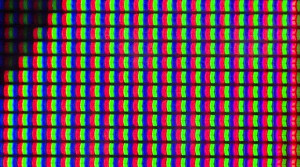
\includegraphics[scale=0.5]{Images/pixel.jpg}
 \caption{Représentation des pixels}
  \end{figure}
  
 Maintenant que nous avons expliqué le principe du système RGB, nous allons expliquer son application sur une image. Étant donné la nature du système RGB, celui-ci est donc représenté par la superposition de trois valeurs comprises entre 0 et 255. Chaque valeur représentant l'intensité associée à sa couleur primaire. L'image couleur est donc informatiquement une superposition de trois matrices.
 \begin{figure}[H]
 \centering
 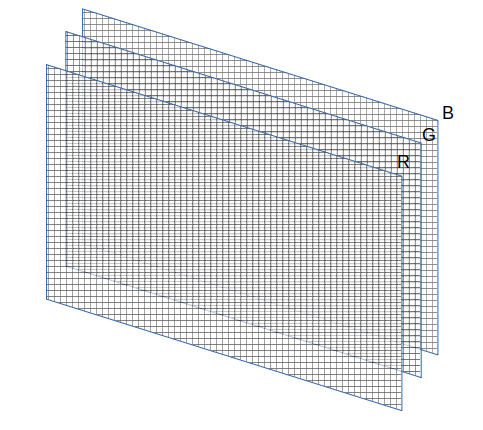
\includegraphics[scale=0.2]{Images/rgb.png}
 \caption{Superposition des matrices}
 \end{figure}
 
  L'image ci-dessous représente bien les possibilités que l'on peut obtenir en superposant les couleurs (si toutes les valeurs sont nulles on obtient du noir, si toutes les valeurs sont 255 on obtient du blanc, etc...).
 
 \begin{figure}[H]
 \centering
 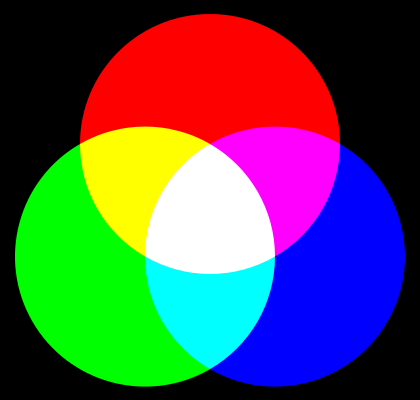
\includegraphics[scale=0.3]{Images/RGB.png}
 \caption{Superposition des couleurs}
  \end{figure}
 
Afin de résoudre le problème sur des images en couleur, nous avons donc appliqué les mêmes algorithmes que nous avions utilisé pour une image en niveau de gris, sur chacune des matrices associée aux couleurs primaires.\newline
 
La couleur de l'objet à coller est donc souvent "dénaturée".\\
Afin de résoudre ce problème nous aurions pu utiliser un autre espace de couleurs, l'espace HSL (Hue Saturation Lightness ou Teinte Saturation luminosité en français), ce système est plus éloigné de la machine, mais plus près de la perception de l'homme. En effet, l'œil ne perçoit pas la couleur comme une superposition de couleurs, mais comme une sensation de luminosité. La saturation représente "l'intensité" de la couleur (si la couleur est plus ou moins forte), la teinte représente les différentes couleurs possibles dues aux mélanges de couleurs primaires et enfin la luminosité est remarquable selon si une image est plus ou moins sombre (proche du blanc ou du noir). La teinte est représentée par une valeur modulo 360, la saturation est une valeur entre 0 (sensation peu coloré) et 1 (sensation très coloré) et la luminosité est une valeur entre 0 et 1 représentant le pourcentage de luminosité.
\begin{figure}
\centering
 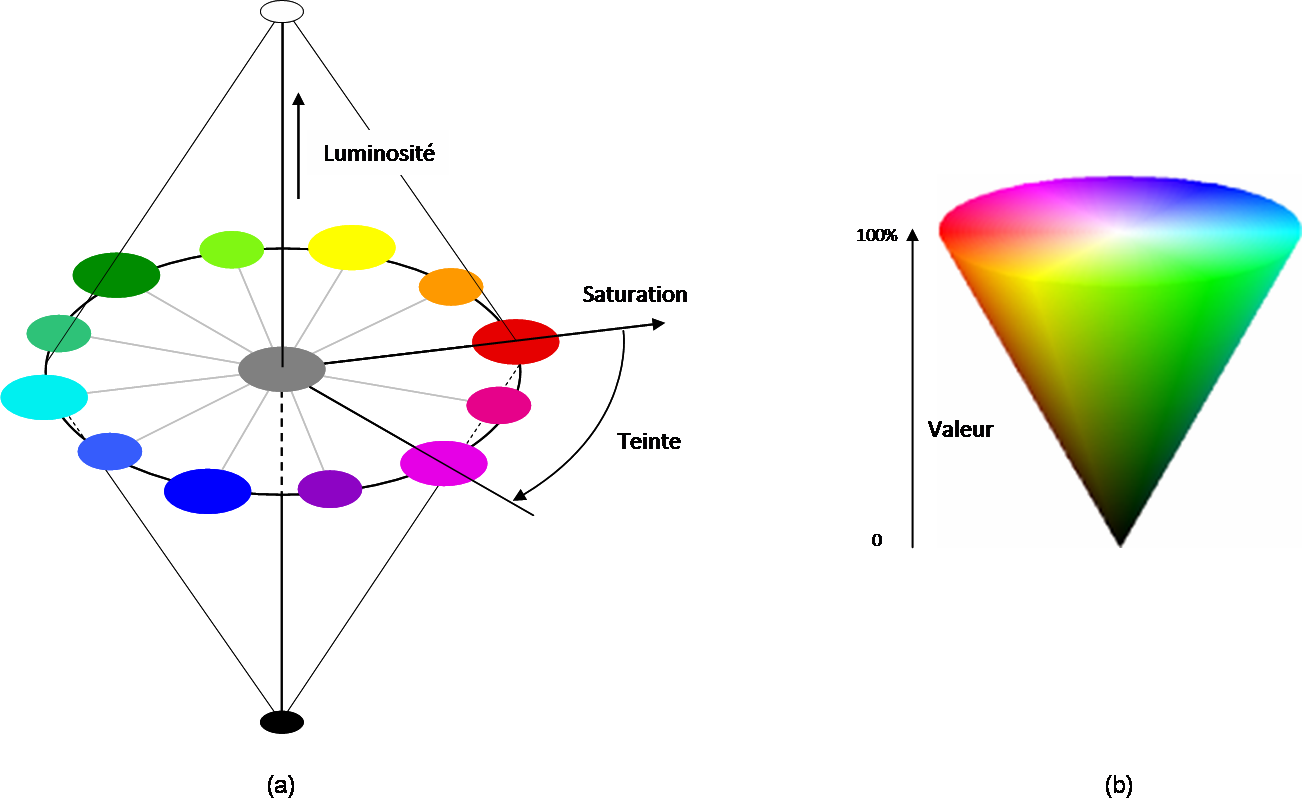
\includegraphics[scale=0.5]{Images/TSL.png}
 \caption{Système HSL}
\end{figure}
 
 Il y a une grande différence entre le nombre de couleurs que peut percevoir l'homme et le nombre de couleurs qui existent, en effet l'œil ne peut percevoir que jusqu'à un demi million de couleurs différentes, alors que, par exemple le système RGB peut fournir $255^3$ couleurs (soit environ 16 millions), il y a donc beaucoup de couleurs qui selon la machine sont différentes mais que l'homme ne peut différenciées.
